\documentclass[compress]{beamer}

\usetheme{Hamburg}

\usepackage[T1]{fontenc}
\usepackage[utf8]{inputenc}

\usepackage{lmodern}

\usepackage[english]{babel}
%\usepackage[ngerman]{babel}

\usepackage{eurosym}
\usepackage{listings}
\usepackage{microtype}
\usepackage{units}
\usepackage{hyperref}
\usepackage{url}


\lstset{
	basicstyle=\ttfamily\footnotesize,
	frame=single,
	numbers=left,
	language=C,
	breaklines=true,
	breakatwhitespace=true,
	postbreak=\hbox{$\hookrightarrow$ },
	showstringspaces=false,
	tabsize=4,
	captionpos=b,
	morekeywords={gboolean,gpointer,gconstpointer,gchar,guchar,gint,guint,gshort,gushort,glong,gulong,gint8,guint8,gint16,guint16,gint32,guint32,gint64,guint64,gfloat,gdouble,gsize,gssize,goffset,gintptr,guintptr,int8_t,uint8_t,int16_t,uint16_t,int32_t,uint32_t,int64_t,uint64_t,size_t,ssize_t,off_t,intptr_t,uintptr_t,mode_t}
}

\title{I/O analysis of climate applications}
\author{Arne Beer \& Frank Röder}
\institute{Arbeitsbereich Wissenschaftliches Rechnen\\Fachbereich Informatik\\Fakultät für Mathematik, Informatik und Naturwissenschaften\\Universität Hamburg}
\date{2016-07-7}

\titlegraphic{
\includegraphics[width=0.75\textwidth]{gfx/logo}}

\begin{document}

\begin{frame}
	\titlepage
\end{frame}

\begin{frame}
	\frametitle{Content (Agenda)}

	\tableofcontents[hidesubsections]
\end{frame}

\section{Introduction}
\begin{frame}
	\frametitle{Introduction}
\begin{itemize}
	\item what climate models do
	\item what is important about them
	\item take a look at the workflow (especially pre- and post-processing)
	\item take a look at storage systems
	\item deliver knowledge about that
\end{itemize}

\end{frame}

\subsection{Goals and Tasks}
\begin{frame}
	\frametitle{Goals and Tasks}
	
\begin{itemize}
	\item try to run models
	\item analyze their input and output
	\item take a look at the live-cycle of data
	\item deliver knowledge about that
\end{itemize}

\end{frame}

\section{Models and Research}
\begin{frame}
    \frametitle{The Models}

    \begin{itemize}
    	\item IFS
	\item AWIPS II
	\item CESM
	\item ECHAM
    \end{itemize}

\end{frame}

\section{Awips II}
\begin{frame}
    \frametitle{Awips II}
    \begin{center}
    	\begin{figure}
			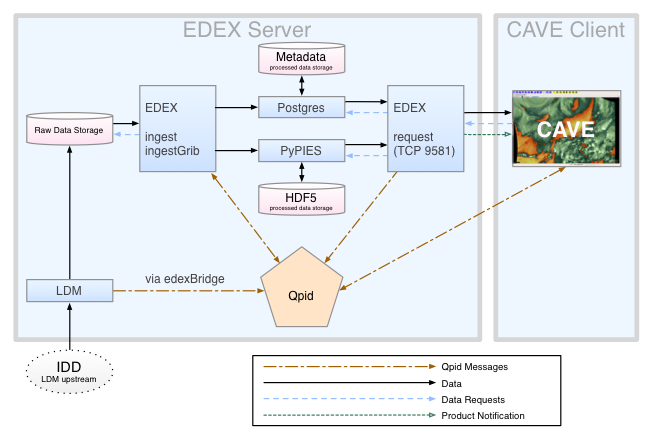
\includegraphics[width=0.7\textwidth]{gfx/awipsII.png}
      	  	\caption[]{Awips Infrastructure \cite{Uni01}}
		\end{figure}
	\end{center}

\end{frame}

\section{CESM}
\begin{frame}
    \frametitle{CESM}
    	\begin{itemize}
    	    \item Community Earth System Model
			\item model for global climate simulation
			\item covers atmosphere, land, land ice, sea ice, ocean and river
			\item provides scripts for setting up the machine in 4 commands
	    	\begin{itemize}
		    	\item scripts are broken
		    	\item mix of bash, csh, perl
		    \end{itemize}
		    \item good configurability with xml files
		    \item requires netCDF format for input data \cite{CESMDocs}
		\end{itemize}
\end{frame}

\subsection{Input and Output analysis}
\begin{frame}[fragile]
	\frametitle{I/O analysis}


\end{frame}




\section{Summary}

\begin{frame}
	\frametitle{Summary}

	\begin{itemize}
		\item Models
		\begin{itemize}
			\item CESM, ECHAM
		\end{itemize}

		\item Data
		\begin{itemize}
			\item life-cycle
			\item pre- and post-processing
		\end{itemize}
		\item analyzing
		\begin{itemize}
		    \item AWIPS II
		\end{itemize}
	\end{itemize}
\end{frame}

\section*{Literature}

\begin{frame}[allowframebreaks]
	\frametitle{Literature}
    \frametitle{Sources}

	\bibliographystyle{alpha}
	\bibliography{literatur.bib}
\end{frame}

\end{document}
